\documentclass[conference]{IEEEtran}

% --- Packages ---
\usepackage[utf8]{inputenc}
\usepackage[T1]{fontenc}
\usepackage{amsmath,amssymb,amsfonts}
\usepackage{graphicx}
\usepackage{subcaption}
\usepackage{booktabs}
\usepackage{url}
\usepackage[hidelinks]{hyperref}

% --- Paper metadata ---
\title{Predicting Ride Fare Prices with Machine Learning\\
\large Uber \& Lyft Regression Analysis}

\author{%
\IEEEauthorblockN{Michael DeJournett}
\IEEEauthorblockA{University of Nebraska-Lincoln\\
\texttt{mdejournett2@unl.edu}}
\and
\IEEEauthorblockN{Hugh Strumberger}
\IEEEauthorblockA{University of Nebraska-Lincoln\\
\texttt{hstrumberger2@unl.edu}}
}
\begin{document}

\maketitle

\begin{abstract}
This report predicts Uber and Lyft fares with supervised learning.
We use 14 features from each trip, including distance, time, location, vehicle type, and weather.
We compare Linear Regression and Random Forest using MAE, RMSE, $R^2$, confidence intervals, and normalized confusion matrices.
Random Forest performs best with MAE = \textbf{\$1.30}, RMSE = \textbf{\$2.32}, and $R^2=\textbf{0.939}$.
Its 95\% MAE confidence interval is \textbf{[1.238, 1.380]}.
Overall, Random Forest gives better accuracy and more stable results than the linear baseline on this dataset.
\end{abstract}

\begin{IEEEkeywords}
machine learning, regression, random forest, Uber, Lyft, fare prediction
\end{IEEEkeywords}

\section{Introduction}
Fare prediction helps riders understand prices and helps companies plan service.
In this project, we compare a simple linear model and an ensemble model on Uber/Lyft trip data.
The best results are MAE = \textbf{\$1.30}, RMSE = \textbf{\$2.32}, and $R^2=\textbf{0.939}$.
We also report 95\% confidence intervals from repeated holdout splits.
Random Forest is the best model for this dataset, so we select it as the final model.
The rest of the paper explains the problem, methods, results, and limits of the approach.

\section{Problem Formulation}
The task is to predict ride fare price in USD from 14 trip and context features.
Inputs include distance in miles, time features such as hour, day of week, and month, pickup and drop-off locations,
vehicle type information such as cab type and service name, and weather conditions such as temperature, humidity, wind, pressure, rain, and clouds.
The output is one value: the trip fare.
We evaluate with repeated 80\%/20\% train-test holdout over 20 runs.
For preprocessing, we fill missing numeric values using medians from the training split and encode categories with training-split mappings.
We scale features for Linear Regression and keep unscaled features for Random Forest.
We intentionally exclude \texttt{surge\_multiplier} from training.
It is very close to a direct pricing signal, so including it can act like using price information to predict price.
In early runs, this feature dominated the models and made many metrics look artificially strong.
That made comparison less useful because both models were driven by the same near-direct signal rather than broader trip and weather patterns.

\section{Models}
Two main models are compared:
\begin{itemize}
\item \textbf{Linear Regression Baseline:} A standard least-squares model with StandardScaler.
          We use it as a simple and easy-to-explain baseline.
\item \textbf{Random Forest Regressor Ensemble:} 30 trees with max depth 10 and random state 42.
		  This model can learn non-linear patterns and feature interactions.
\end{itemize}
We do not run full hyperparameter tuning.
These settings were chosen to balance model quality and runtime.

\section{Performance Indicators and Best Model Justification}
We compare models using these regression metrics:
\begin{itemize}
	\item Mean Absolute Error (MAE)
	\item Root Mean Squared Error (RMSE)
	\item Coefficient of Determination ($R^2$)
\end{itemize}
We also report 95\% confidence intervals.

\begin{table}[htbp]
\caption{Model Performance with Repeated Holdout (20 Splits) and 95\% Confidence Intervals}
\label{tab:results}
\centering
\begin{tabular}{lccc}
\toprule
Model & MAE (95\% CI) & RMSE (95\% CI) & $R^2$ (95\% CI) \\
\midrule
Linear Regression & 6.58 [5.012, 7.136] & 8.21 [6.675, 8.768] & 0.233 [0.130, 0.493] \\
Random Forest & \textbf{1.30 [1.238, 1.380]} & \textbf{2.32 [2.125, 2.466]} & \textbf{0.939 [0.932, 0.948]} \\
\bottomrule
\end{tabular}
\end{table}

\section{Normalized Confusion Matrix for Binned Fares}
The main task is regression, but we also bin fares into low, medium, and high ranges.
This lets us build normalized confusion matrices to show how often each fare range is predicted correctly.
Row-normalized confusion matrices for both Linear Regression and Random Forest are shown below.

\begin{figure}[htbp]
\centering
\subfloat[Linear Regression]{%
\IfFileExists{figures/normalized_confusion_matrix_lr.png}{
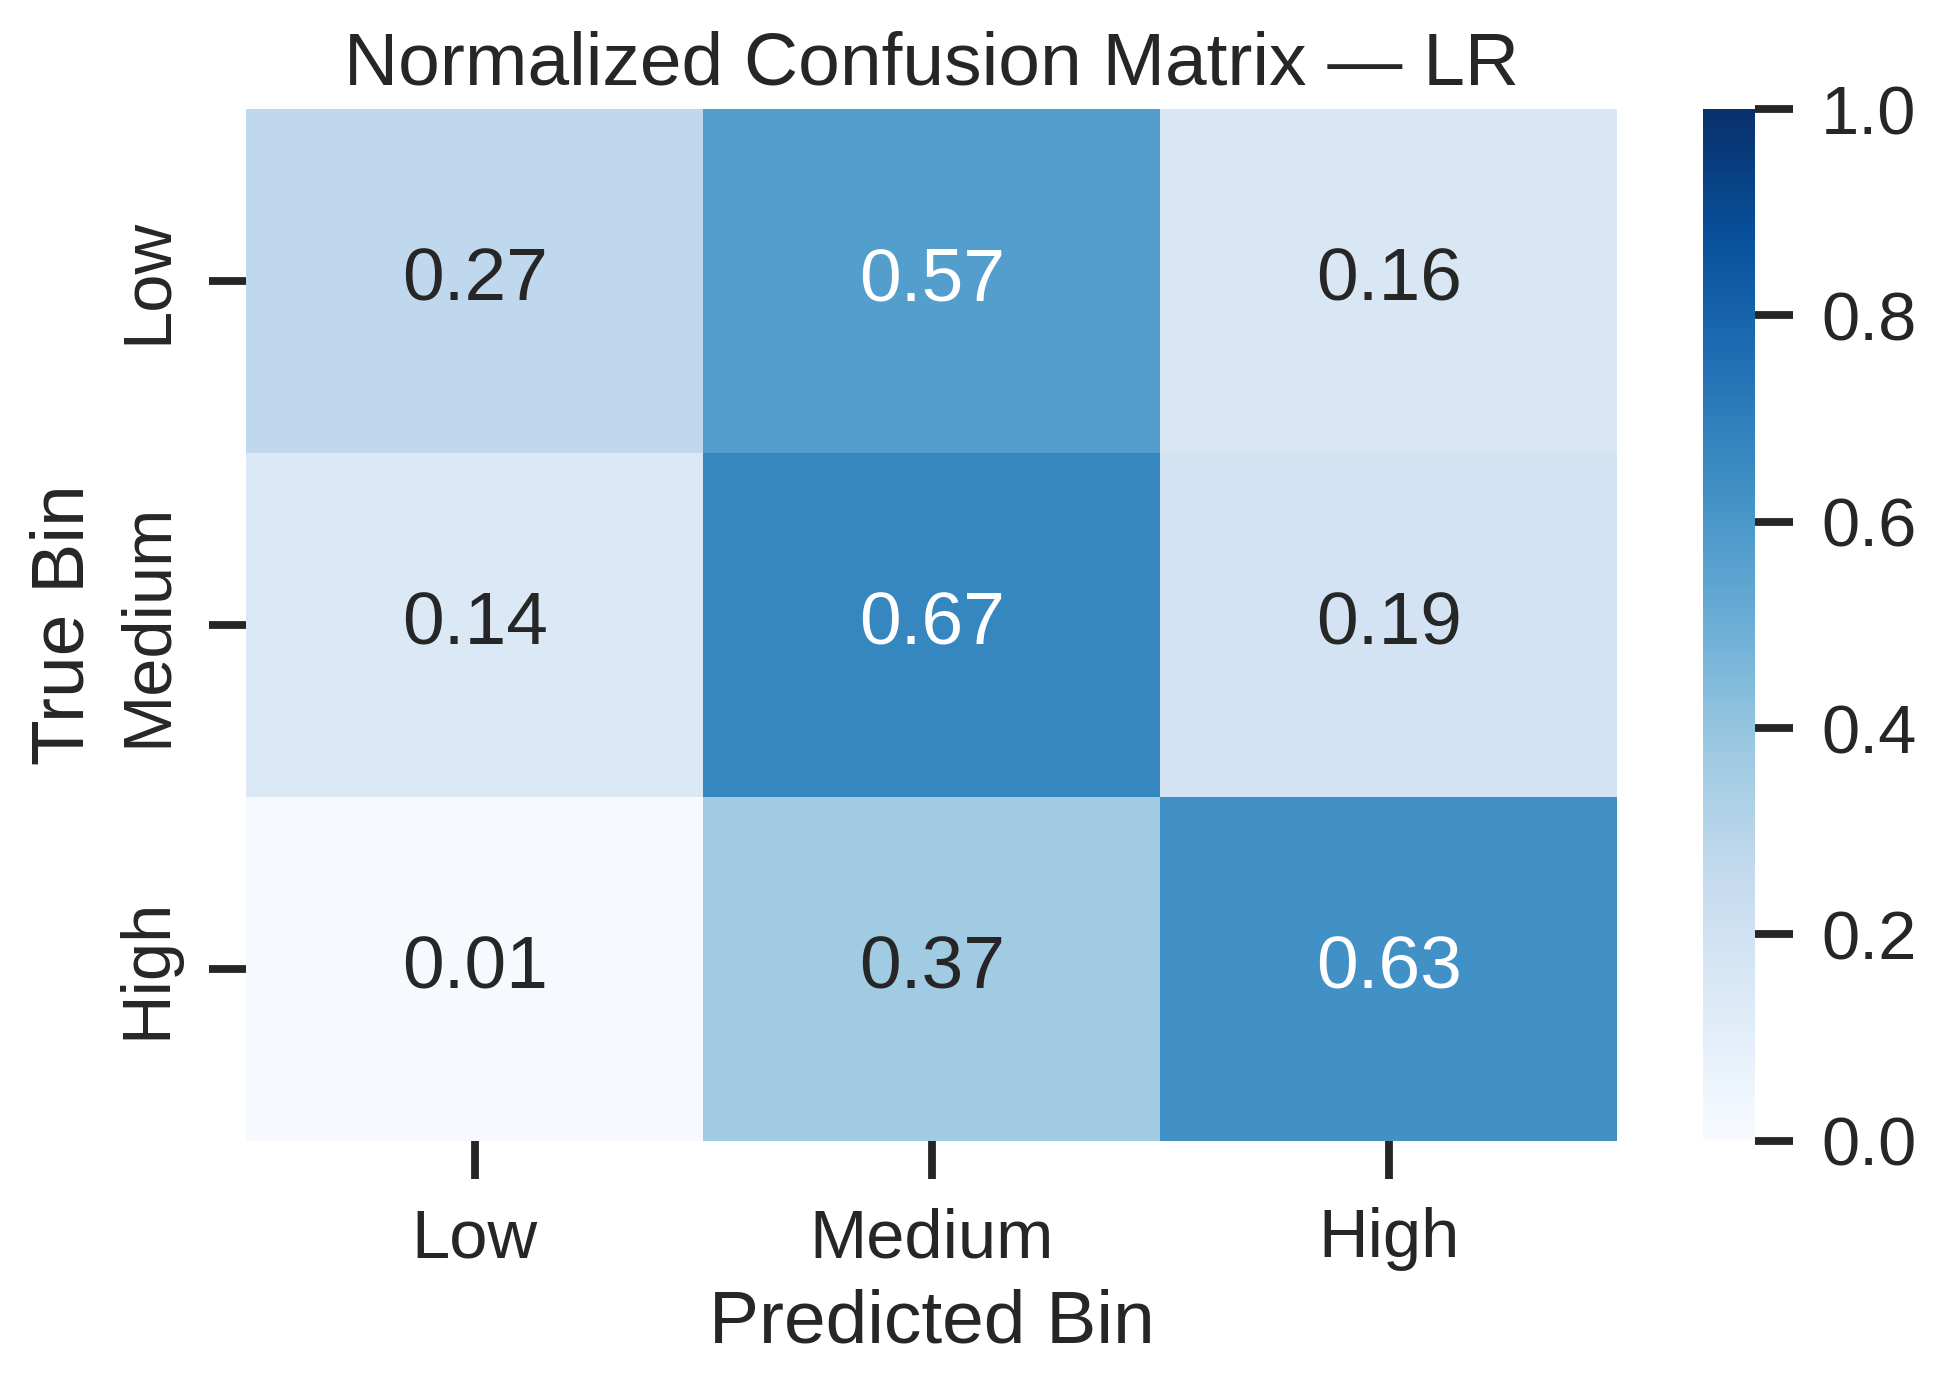
\includegraphics[width=0.45\columnwidth]{figures/normalized_confusion_matrix_lr.png}
}{
\fbox{\parbox[c][2.5cm][c]{0.43\columnwidth}{\centering LR matrix}}
}
}%
\hspace{0.05\columnwidth}%
\subfloat[Random Forest]{%
\IfFileExists{figures/normalized_confusion_matrix_rf.png}{
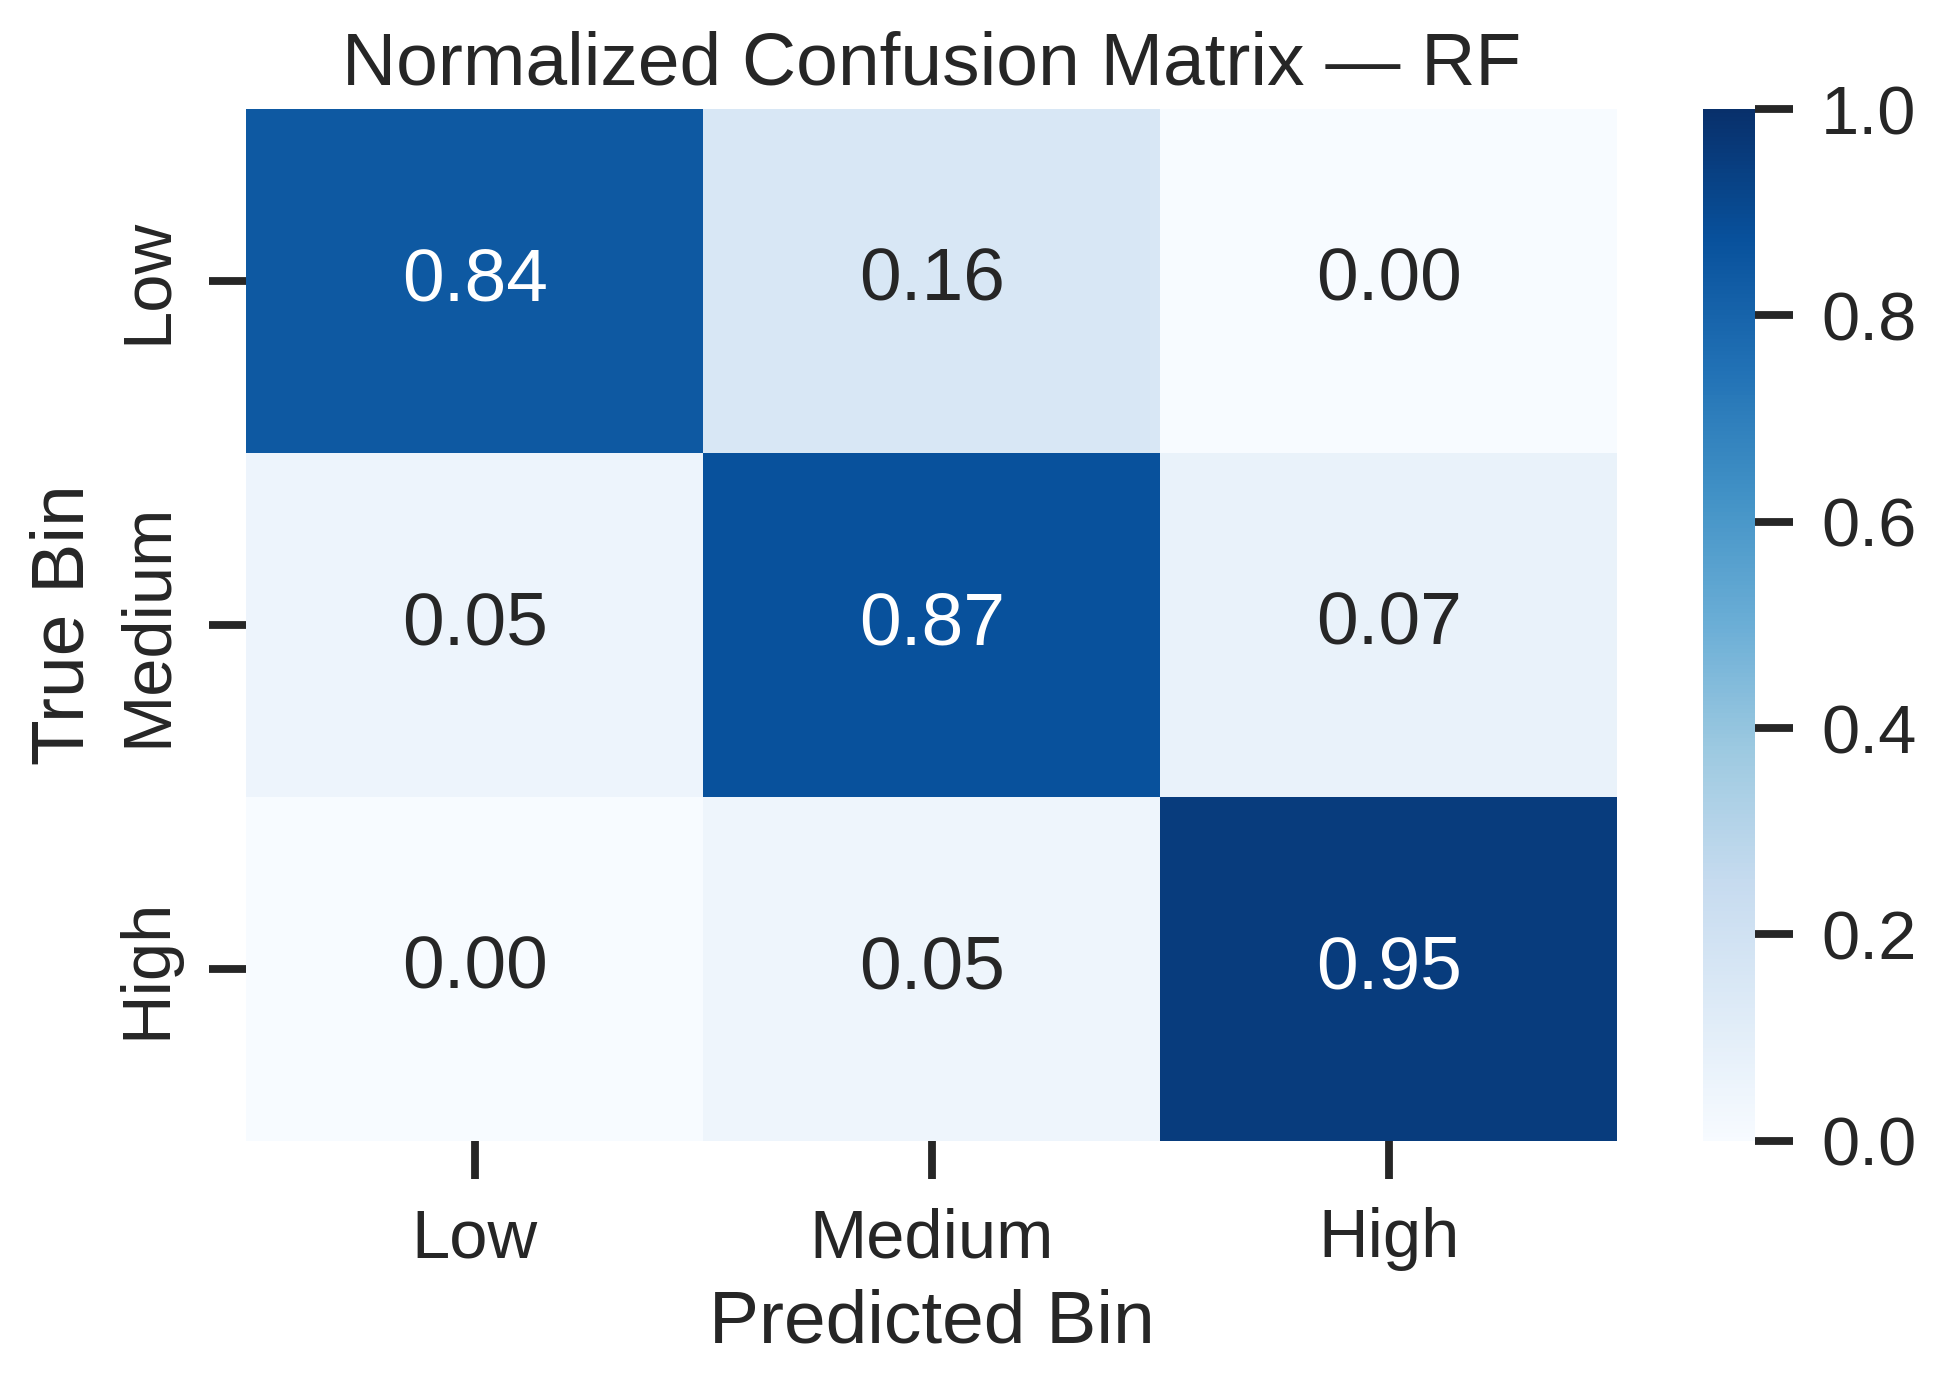
\includegraphics[width=0.45\columnwidth]{figures/normalized_confusion_matrix_rf.png}
}{
\fbox{\parbox[c][2.5cm][c]{0.43\columnwidth}{\centering RF matrix}}
}
}
\caption{Normalized confusion matrices on binned fare ranges for both models.}
\label{fig:ncm}
\end{figure}
In these matrices, stronger values on the diagonal mean the model is correctly placing trips in the right fare range.
The Random Forest matrix has a stronger diagonal and weaker off-diagonal values, so it confuses fare ranges less often than Linear Regression.

\section{Actual vs Predicted Analysis}
These scatter plots compare true fares with predicted fares.
Linear Regression shows larger and more systematic errors.
Random Forest points are closer to the diagonal line, which means better predictions.

\begin{figure}[htbp]
\centering
\IfFileExists{figures/actual_vs_predicted.png}{
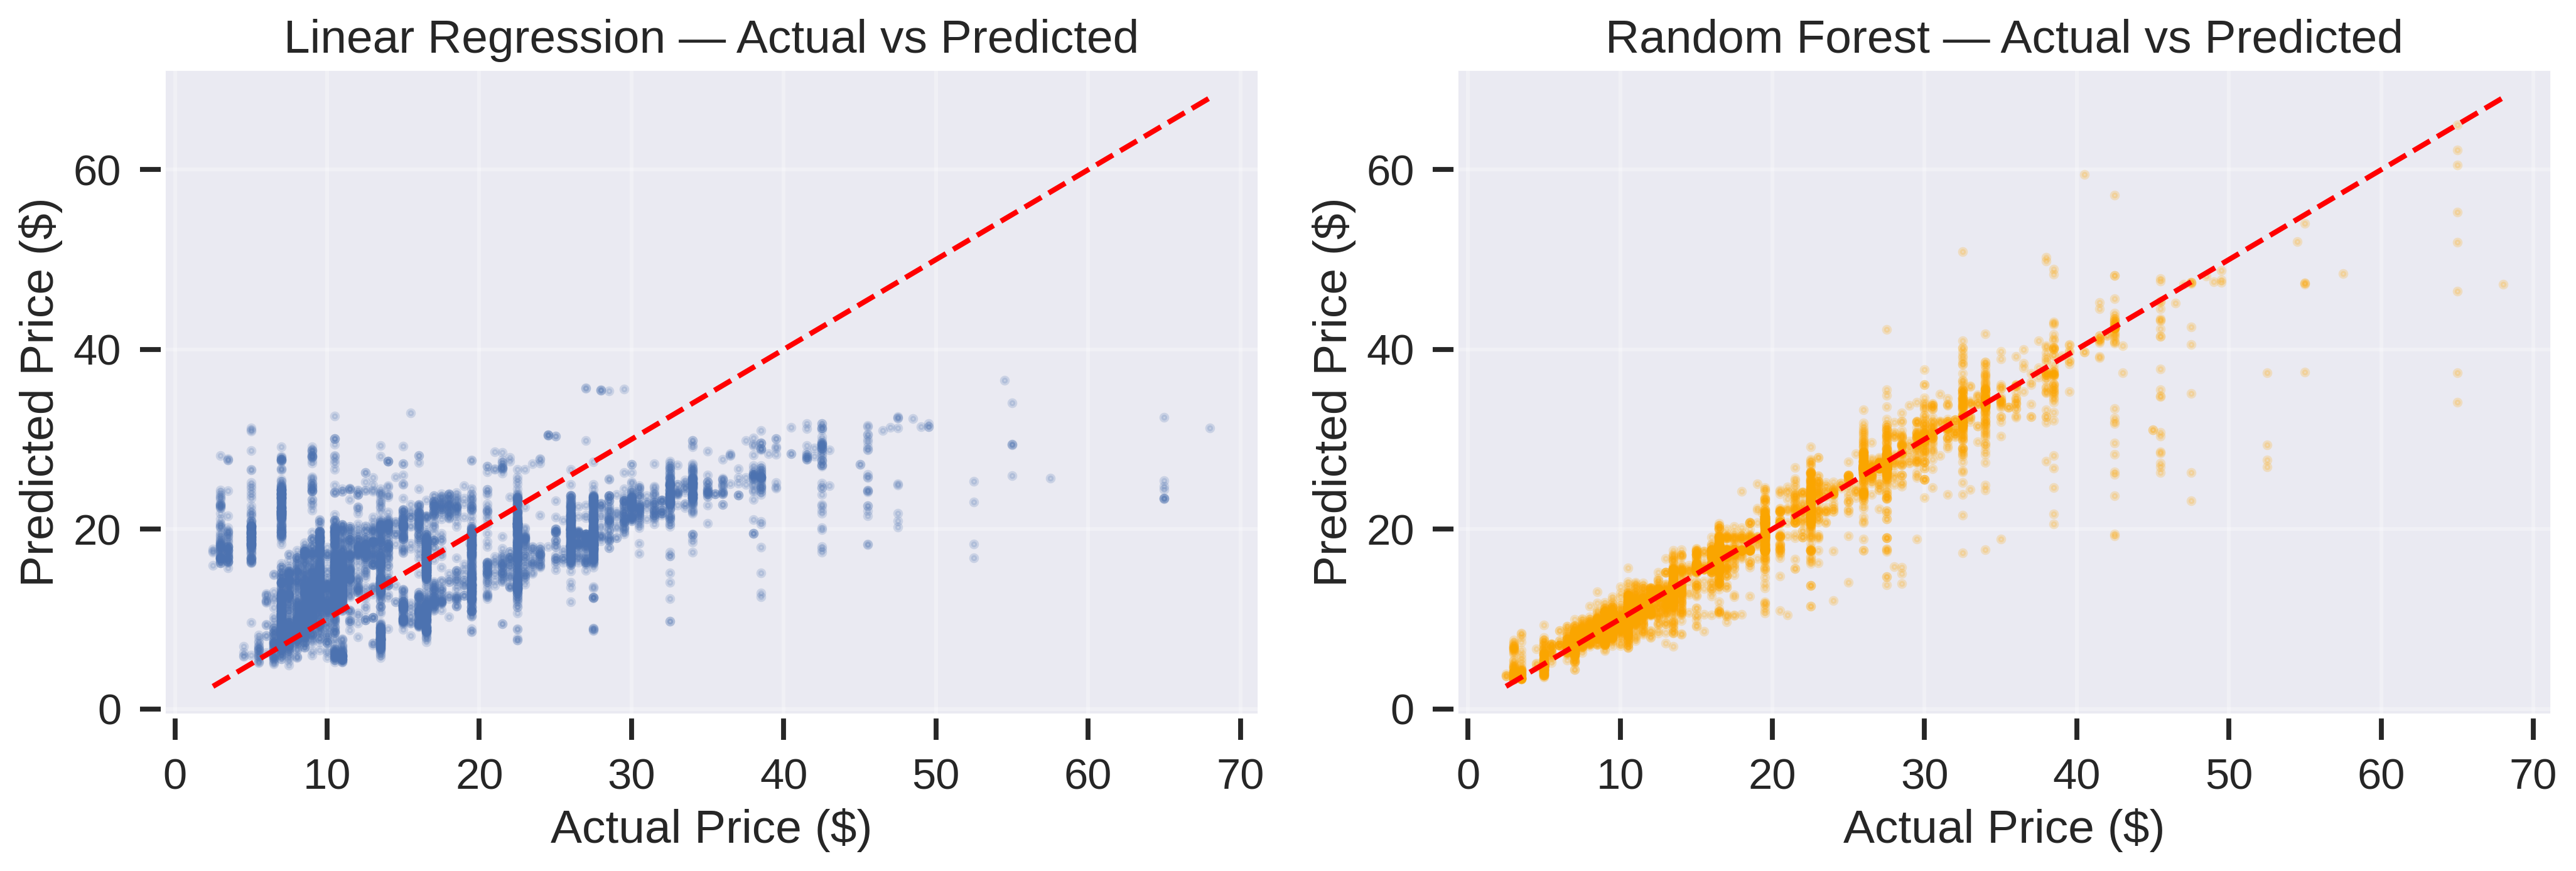
\includegraphics[width=0.85\columnwidth]{figures/actual_vs_predicted.png}
}{
\fbox{\parbox[c][3cm][c]{0.83\columnwidth}{\centering Actual vs Predicted Plots}}
}
\caption{Actual vs Predicted scatter plots for both Linear Regression (left) and Random Forest (right).
The diagonal dashed line represents perfect predictions. Random Forest concentrates much more tightly around this line.}
\label{fig:avp}
\end{figure}
This figure shows prediction error size and pattern.
Points far from the diagonal are larger errors, while points close to the diagonal are better predictions.
Because Random Forest points cluster closer to the diagonal across low and high fares, it has lower overall error.

\section{Feature Importance Comparison}
Feature importance helps us see which inputs matter most.
Linear Regression coefficients show linear effects.
Random Forest importances show how useful each feature is when making tree-based decisions.

\begin{figure}[htbp]
\centering
\IfFileExists{figures/feature_importance.png}{
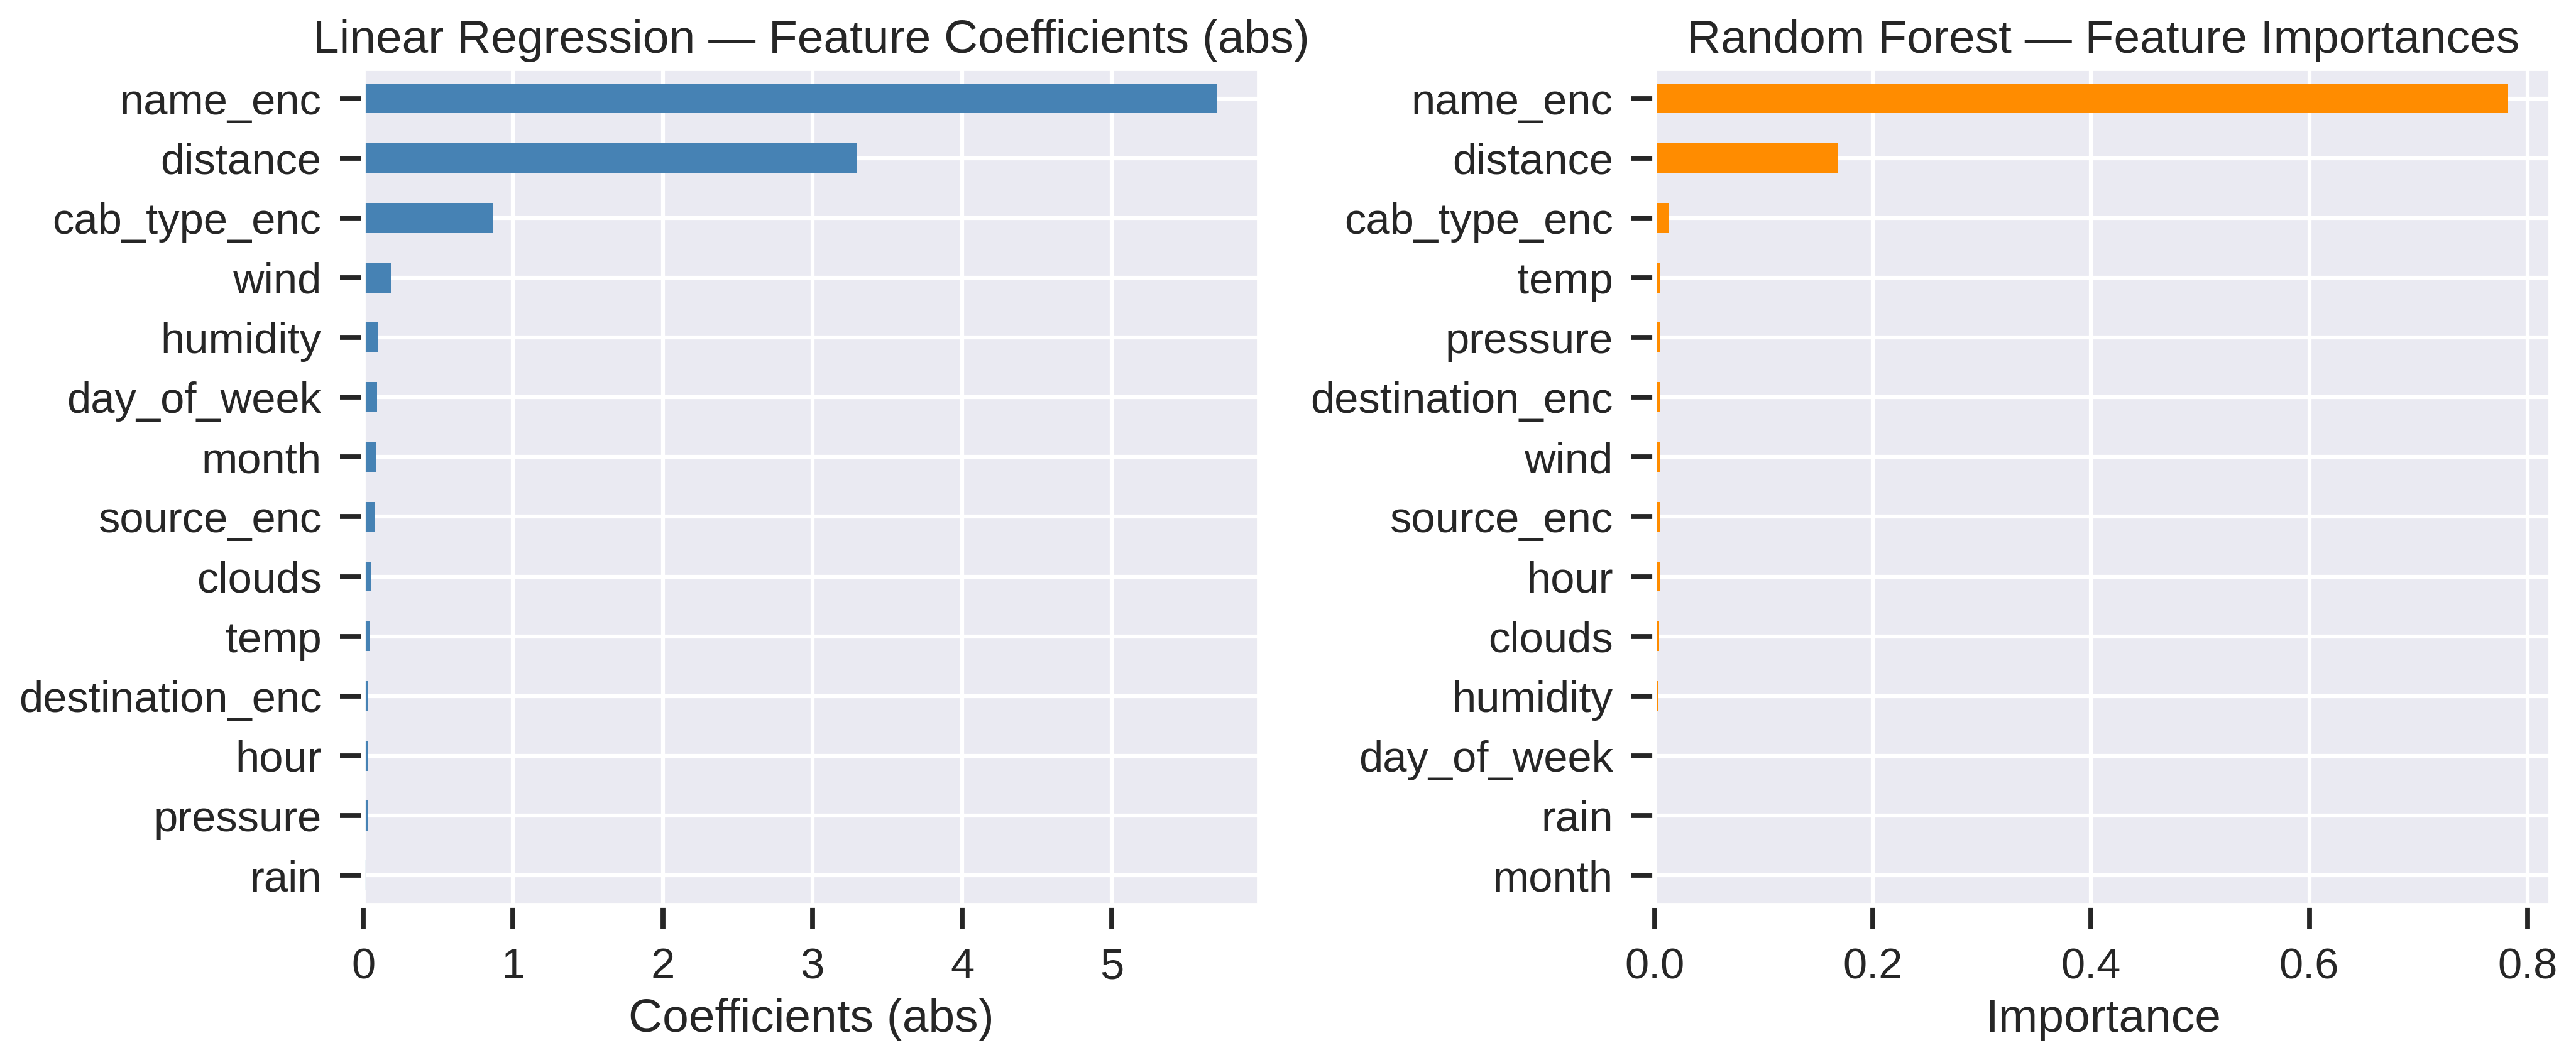
\includegraphics[width=0.85\columnwidth]{figures/feature_importance.png}
}{
\fbox{\parbox[c][3cm][c]{0.83\columnwidth}{\centering Feature Importance}}
}
\caption{Feature importance comparison: Linear Regression absolute coefficients (left, steel blue) vs.
Random Forest feature importances (right, dark orange). Both models rank service type and distance as top predictors,
validating domain knowledge about ride fare drivers.}
\label{fig:fi}
\end{figure}
This figure explains \emph{why} the models make their predictions.
Features with larger bars have a stronger effect on output, and both models highlight distance and service-related fields as key drivers of fare.

\section{Model Comparison Summary}
The two models differ in both simplicity and predictive power.
Linear Regression is easier to interpret because it uses one global equation.
Each coefficient has a direct and consistent meaning across samples:
\begin{equation}
\hat{y}=w_0+\sum_j w_j x_j.
\end{equation}
This makes it easy to explain why a prediction changes when one input changes.
Random Forest is harder to interpret, but it captures complex non-linear patterns.
For this application, the $R^2$ improvement from 0.233 to 0.939 and MAE reduction from \$6.58 to \$1.30
justify the shift toward the ensemble method.

\section{Pros and Cons by Model}
\textbf{Linear Regression (Baseline)}

\textbf{Pros:}
\begin{itemize}
	\item Simple and easy to interpret.
	\item Fast to train and evaluate.
	\item Good transparent baseline for comparison.
\end{itemize}

\textbf{Cons:}
\begin{itemize}
	\item Lower predictive performance on this dataset (MAE = \$6.58, $R^2$ = 0.233).
	\item Does not model complex non-linear interactions well.
\end{itemize}

\textbf{Random Forest (Ensemble)}

\textbf{Pros:}
\begin{itemize}
	\item Best predictive performance on this dataset (MAE = \$1.30, $R^2$ = 0.939).
	\item Captures non-linear feature interactions.
	\item Less sensitive to feature scaling.
\end{itemize}

\textbf{Cons:}
\begin{itemize}
	\item Harder to interpret than Linear Regression.
	\item Can still be affected by data quality and sampling.
\end{itemize}

\section{Conclusion}
Random Forest gives the best overall performance on this Uber/Lyft dataset.
It explains 93.9\% of fare variance and reaches a mean absolute error of \$1.30.
We still include Linear Regression as a clear baseline for comparison.
We also exclude \texttt{surge\_multiplier} on purpose so the comparison reflects general trip and weather signals instead of a near-direct pricing input.
Future work should test time-based validation and add external signals such as real-time traffic to improve generalization.

\section{Threats to Validity}
We used repeated random train-test splits instead of a time-based split.
Because of that, the results may look better than real-world performance when pricing patterns change over time.
Our confidence intervals are based on variation across those splits.
They are helpful, but they still may not capture all uncertainty in future data.
We also used a sample of 20,000 trips, so rare events may not be fully represented.
That can make errors on unusual cases harder to measure.
Finally, we did not include surge multiplier fields.
So the model predicts fare mostly from trip details and weather, not from direct dynamic-pricing signals.

\end{document}
